\documentclass[aspectratio=169]{slide-en}

\usepackage{physics}
\usepackage{caption}
\usepackage{subcaption}

\usepackage{algorithm}
\usepackage{algpseudocodex}
\usepackage{amsmath}
\usepackage{array}
\usepackage{bbm}
\usepackage{csvsimple} % csvreader

\graphicspath{{src/}{src/rlime-paper/src/}}
\addbibresource{src/rlime-paper/src/ref.bib}

\newcommand{\ispace}{\mathbb{D}^{m}}
\newcommand{\Prec}{\operatorname{acc}}
\newcommand{\Cov}{\operatorname{cov}}
\newcommand{\cands}{\bar{\mathcal{A}}}
\algnewcommand{\IIf}[1]{\State\algorithmicif\ #1\ \algorithmicthen\ }
\renewcommand{\algorithmicrequire}{\textbf{Input:}}
\renewcommand{\algorithmicensure}{\textbf{Output:}}


\newcommand{\dtrain}{D_{\mathrm{train}}}
\newcommand{\dtest}{D_{\mathrm{test}}}
\newcommand{\dmis}{D_{\mathrm{mis}}}
\newcommand{\dchange}{D_{\mathrm{change}}}

\title{\texorpdfstring{
  R-LIME:\@ Rectangular Constraints and Optimization
  for Local Interpretable Model-agnostic Explanation Methods
}{}}
\author{Genji Ohara, Keigo Kimura and Mineichi Kudo}
\date{December 2024}
\institute{%
  Division of Computer Science and Information Technology \\
  Graduate School of Information Sci.\@ and Tech., Hokkaido University \\
  Sapporo 060--0814, JAPAN
}

\begin{document}

\section*{Agenda}

\begin{frame}{}
  \setbeamertemplate{section in toc}[ball unnumbered]
  \setcounter{tocdepth}{1} % show only chapters and sections in toc
  \tableofcontents
\end{frame}

\section{Background}
\begin{frame}{}
  \colorrect{red!30}{Interpretable Machine Learning}
  \bigskip
  \begin{columns}[]
    \begin{column}{0.5\textwidth}
      \begin{itemize}
        \item Complex ML models (Black Box)
              \begin{itemize}
                \item Deep Neural Networks
                \item Ensemble Models
              \end{itemize}
              \smallskip
              \textrightarrow{}Decision process is \underline{unambiguous}
      \end{itemize}
      \centering
      \COLabel{complex}{}
    \end{column}
    \begin{column}{0.5\textwidth}
      \begin{itemize}
        \item Simple ML models (White Box)
              \begin{itemize}
                \item Linear Models
                \item Decision Trees
              \end{itemize}
              \smallskip
              \textrightarrow{}Decision process is \underline{ambiguous}
      \end{itemize}
      \centering
      \COLabel{simple}{}
    \end{column}
  \end{columns}
  \begin{tikzpicture}[remember picture,overlay]
    \draw (simple) edge [->, thick, bend left=20] node [midway, below]
      {\colorrect{blue!30}{Approximate Locally}} (complex);
  \end{tikzpicture}
\end{frame}

\section{Related Work}

\begin{frame}{}
  \begin{itemize}
    \item LIME\footfullcite{ribeiro2016why}
    \item Anchor\footfullcite{ribeiro2018anchors}
  \end{itemize}
\end{frame}

\subsection{LIME}

\begin{frame}{}
  Related Work 1 — \textbf{LIME
    \small{(Local Interpretable Model-agnostic Explanations)}}
  \footfullcite{ribeiro2016why}
  \begin{columns}[]
    \begin{column}{0.5\textwidth}
      \begin{enumerate}
        \item Generate perturbed instances around the given focal point
        \item Learn a linear model on the perturbed instances
      \end{enumerate}
    \end{column}
    \begin{column}{0.5\textwidth}
      \begin{figure}
        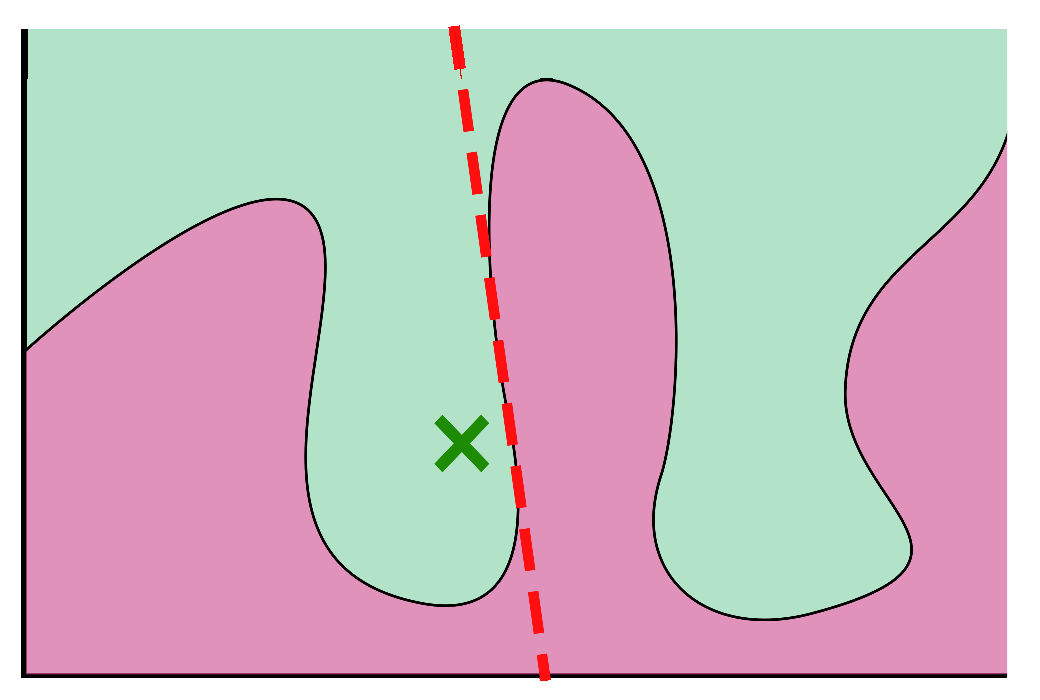
\includegraphics[scale=0.35]{img/visual-lime}
      \end{figure}
    \end{column}
  \end{columns}
\end{frame}

\begin{frame}{}
  \begin{columns}[]
    \begin{column}{0.35\textwidth}
      \vspace{4.2em}
      \begin{figure}
        
\includegraphics[width=\textwidth]{img/example-instance}
        \vspace{0.8em}
        \caption{%
          Example of the focal point.
          The sentiment prediction model predicted this sentence as ``Positive''.
        }
      \end{figure}
    \end{column}
    \begin{column}{0.4\textwidth}
      \begin{figure}
        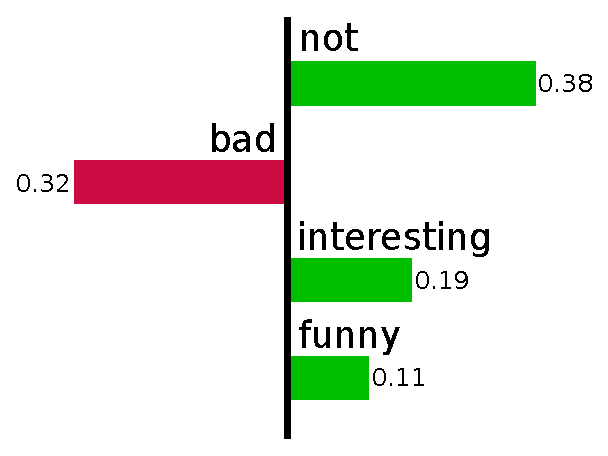
\includegraphics[width=0.9\textwidth]{img/example-lime}
        \caption{%
          Example of LIME's explanation for the output
          by the sentiment prediction model.
        }
      \end{figure}
    \end{column}
  \end{columns}
\end{frame}

\begin{frame}
  \frametitle{Related Work 1 — Drawbacks of LIME}
  \begin{columns}[]
    \begin{column}{0.4\textwidth}
      \underline{Scope of Explanation is Unknown}

      \bigskip
      \begin{itemize}
        \item How general is the knowledge derived from the explanation?
      \end{itemize}
    \end{column}
    \begin{column}{0.45\textwidth}
      \begin{figure}
        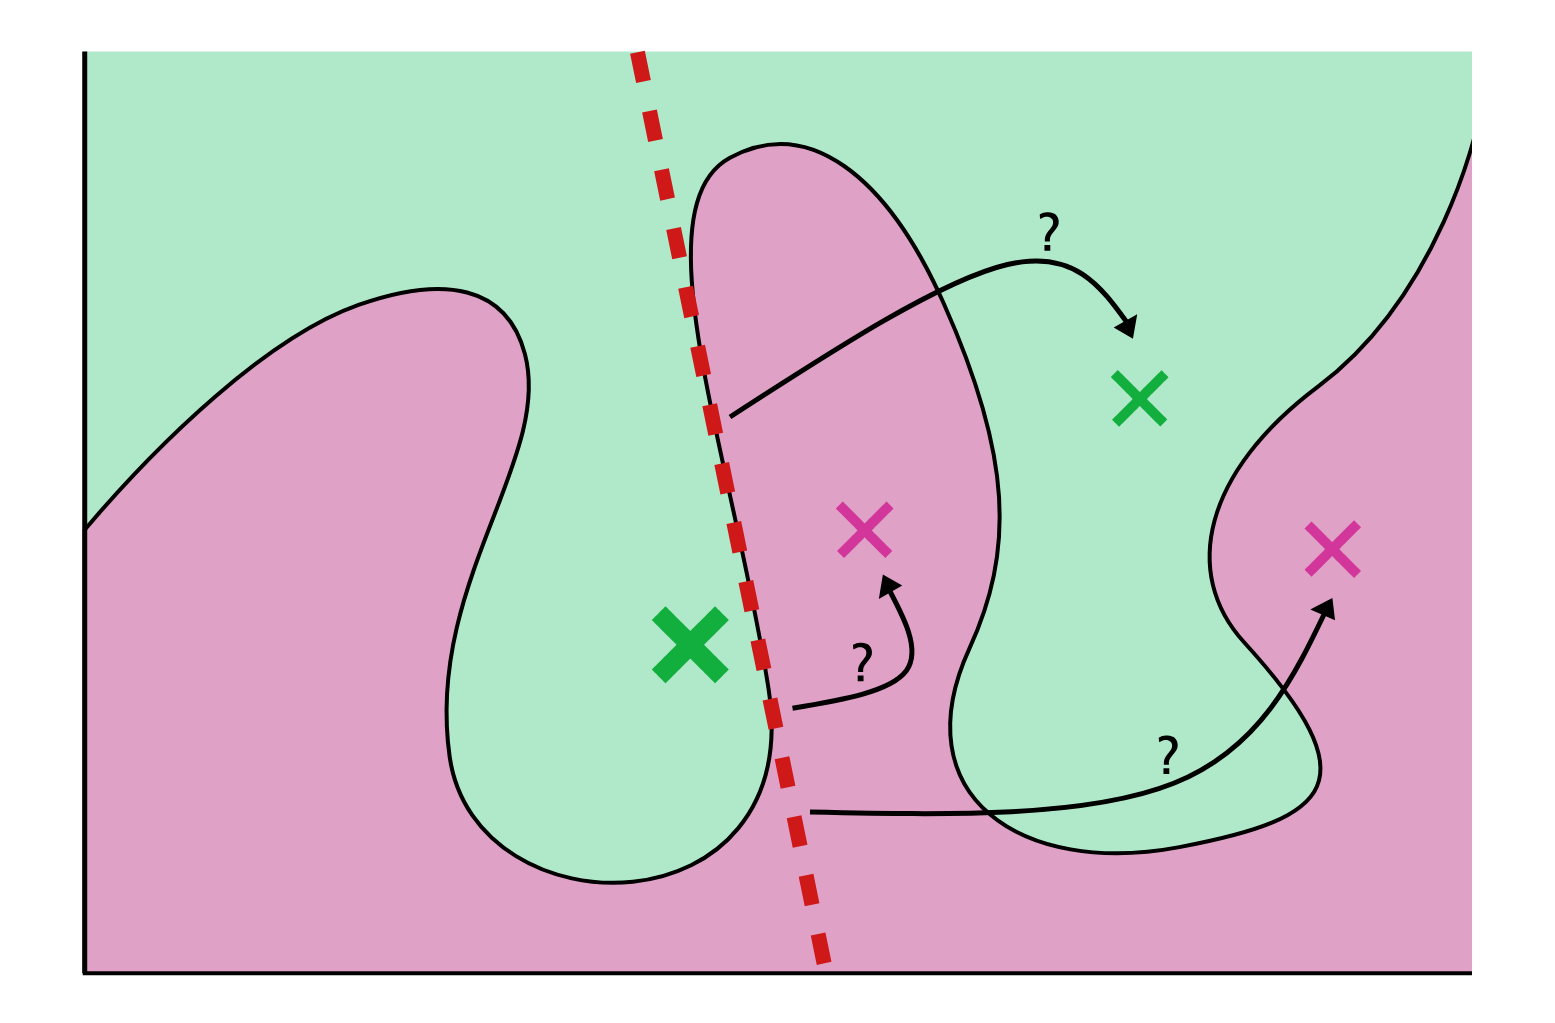
\includegraphics[width=\textwidth]{lime_drawback}
      \end{figure}
    \end{column}
  \end{columns}
\end{frame}

\subsection{Anchor}

\begin{frame}{}
  \begin{columns}[]
    \begin{column}{0.5\textwidth}
      Related Work 2 — Anchor
      \begin{itemize}
        \item Search for the rectangular region in which the model's outputs
              for the focal point and other points are consistent with high
              probability.
        \item Use the feature of the predicate to express the optimal
              rectangular region. \\
              \textit{\footnotesize{ex. Gender = ‘Male’ AND 20 <= Age < 30}}
      \end{itemize}

      \bigskip
    \end{column}
    \begin{column}{0.5\textwidth}
      \begin{figure}
        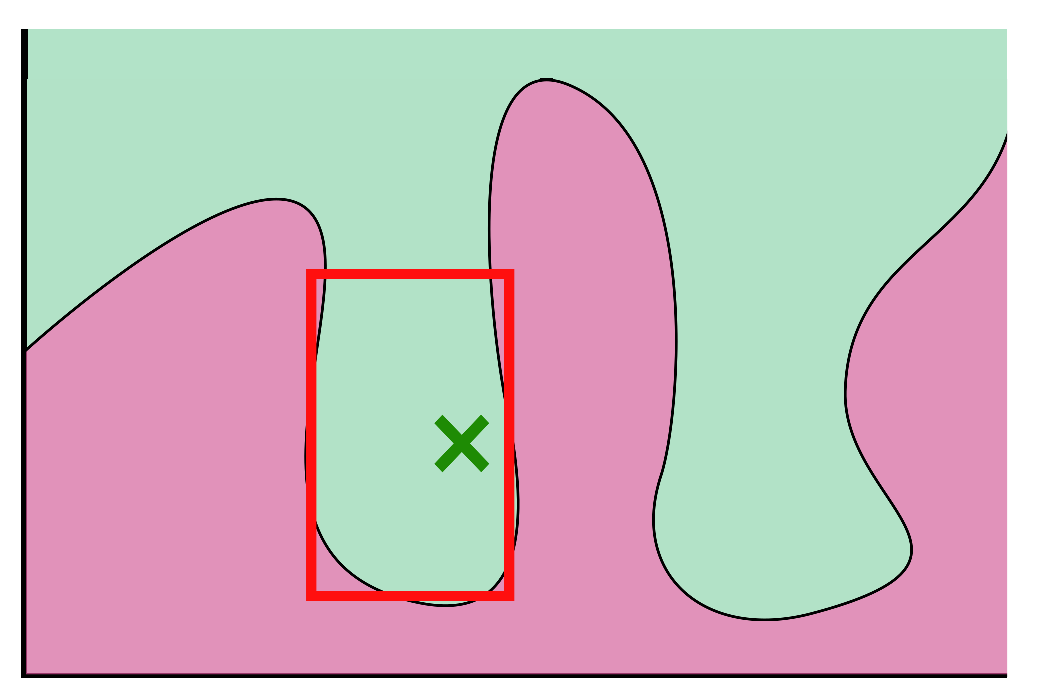
\includegraphics[scale=0.35]{img/visual-anchor}
      \end{figure}
    \end{column}
  \end{columns}
\end{frame}

\subsubsection{Example of Anchor Output}

\begin{frame}{}
  \begin{columns}[]
    \begin{column}{0.35\textwidth}
      \begin{figure}
        \centering
        
\includegraphics[width=\textwidth]{img/example-instance}
        \caption{%
          Example of the focal point.
          The sentiment prediction model predicted this sentence as ``Positive''.
        }
      \end{figure}
    \end{column}
    \begin{column}{0.4\textwidth}
      \vspace{0.7em}
      \begin{figure}
        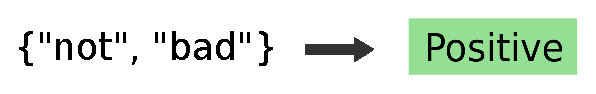
\includegraphics[width=\textwidth]{img/example-anchor}
        \vspace{-0.5em}
        \caption{%
          Example of Anchor explanation for the sentiment prediction model.
        }
      \end{figure}
    \end{column}
  \end{columns}
\end{frame}

\subsubsection{Drawbacks of Anchor}

\begin{frame}{}
  \begin{columns}[]
    \begin{column}{0.45\textwidth}
      \underline{Users get less insight}

      \bigskip
      \begin{itemize}
        \item How much influence does each feature have on the prediction?
      \end{itemize}
    \end{column}
    \begin{column}{0.5\textwidth}
      \begin{figure}
        \begin{subfigure}[t]{\textwidth}
          \centering
          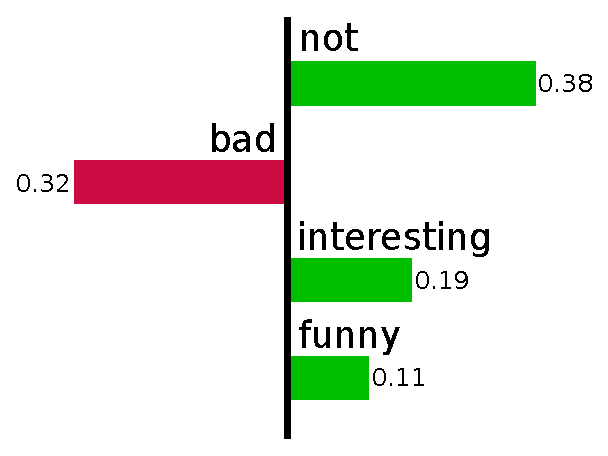
\includegraphics[scale=0.4]{img/example-lime}
        \end{subfigure}
        \begin{subfigure}[t]{\textwidth}
          \centering
          \vspace{0.5em}
          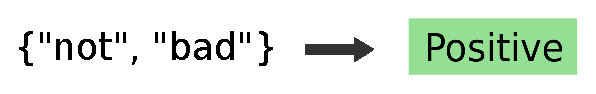
\includegraphics[scale=0.4]{img/example-anchor}
        \end{subfigure}
        \vspace{0.5em}
        \caption{Comparison of LIME and Anchor outputs for the sentiment prediction model}
      \end{figure}
    \end{column}
  \end{columns}
\end{frame}

\subsection{Our Goals}

\begin{frame}{}
  \renewcommand{\arraystretch}{1.5}
  \tabcolsep=1.5em
  \begin{center}
    \begin{tabular}{cccc}
                           & LIME         & Anchor       & Proposed Method \\
      \midrule
      Feature Importance   & \checkmark{} & $\times$     & \checkmark{}    \\
      Optimal Region       & $\times$     & \checkmark{} & \checkmark{}    \\
      Interpretable Region & $\times$     & \checkmark{} & \checkmark{}    \\
    \end{tabular}
  \end{center}

  \bigskip
  Juggle Interpretability of \underline{explanation} and its \underline{region}

  \smallskip
  \textrightarrow{}
  \colorrect{red!20}{%
    Users can utilize knowledge derived from explanation within reasonable range
  }
\end{frame}

\section{Proposed Method: R-LIME}

\begin{frame}{}
  \begin{columns}[]
    \begin{column}{0.45\textwidth}
      \colorrect{red!20}{\textbf{R-LIME (Ruled LIME)} = LIME + Anchor}

      \bigskip
      \begin{itemize}
        \item Approximate in rectangular region
        \item Express the region as a conjunction of feature predicates \\
              \textit{\footnotesize{ex. Gender = ‘Male’ AND 20 <= Age < 30}}
      \end{itemize}
    \end{column}
    \begin{column}{0.55\textwidth}
      \begin{figure}
        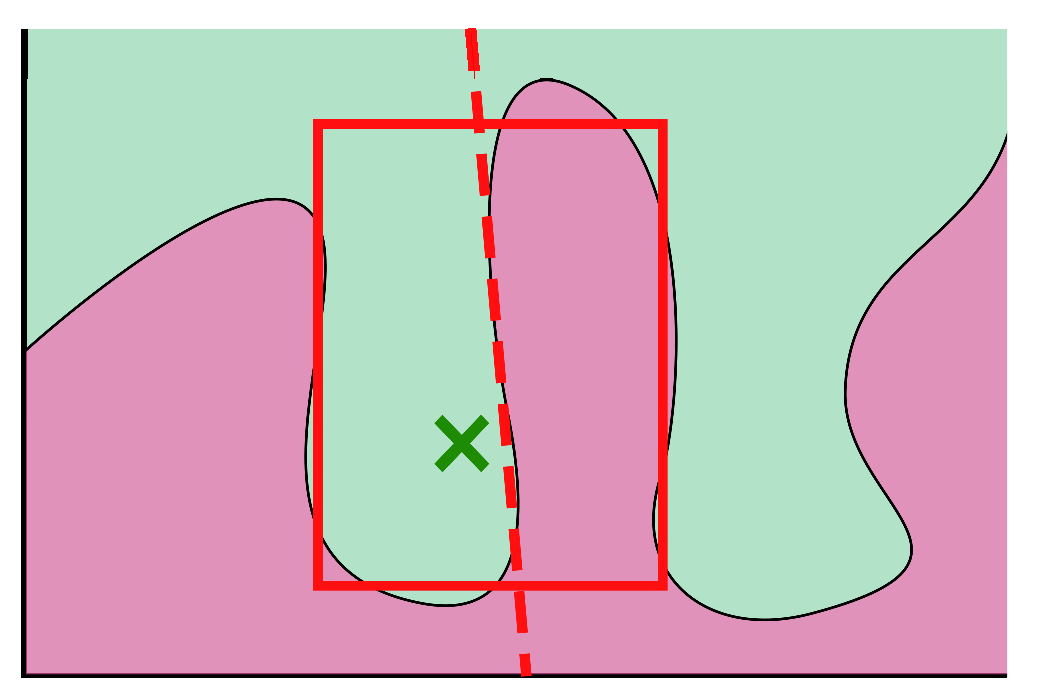
\includegraphics[scale=0.35]{img/visual-rlime3}
      \end{figure}
    \end{column}
  \end{columns}
\end{frame}

\subsection{Setting}

\begin{frame}{}
  \vspace{-1.4em}
  \begin{align*}
     & \text{$m$-dim input space (discretized)}  &  & \ispace             \\
     & \text{A black-box classifier}             &  & f:\ispace\to\{0,1\} \\
     & \text{A focal point}                      &  & x\in\ispace         \\
     & \text{Distribution on input space}        &  & \mathcal{D}         \\
     & \text{Set of all possible approx.\ model} &  & G
  \end{align*}

  \textbf{Rule}: a conjunction of predicates
  \vspace{-0.5em}
  \begin{equation*}
    A(z)=a_{i_1}(z)\wedge a_{i_2}(z)\wedge\dots\wedge a_{i_k}(z),\quad
    a_i(z)=\mathbbm{1}_{z_i=x_i}
  \end{equation*}
\end{frame}

{%
\vfuzz=13.08765pt
\begin{frame}{}
  \bigskip
  \bigskip
  \bigskip

  \begin{alignat*}{2}
     & \text{Accuracy of rule $A$:} & \quad & \Prec(A)=\underset{g\in G}{\max}
    \ \mathbb{E}_{z\sim\mathcal{D}(z|A)}[\mathbbm{1}_{f(z)=g(z)}]
    \COLabel{prec}{}
    \\
     & \text{Coverage of rule $A$:} & \quad & \operatorname{cov}(A)=
    \mathbb{E}_{z\sim\mathcal{D}(z)}[A(z)]
    \COLabel{cov}{}
    \\
    \\
     & \text{Our problem:}          & \quad & \colorrect{red!20}{$
        \tilde{A}=\underset{A\ s.t.
          \ P(\Prec(A)\ge\tau)\ge1-\delta,A(x)=1}  % chktex 36
        {\arg\max}\operatorname{cov}(A)  % chktex 36
      $}
    \COLabel{problem}{}
    \\
  \end{alignat*}

  \begin{center}
    \underline{Maximize coverage under the constraint of accuracy}
  \end{center}
  \CO{prec}{++ (1.0,1.2)}{Expected accuracy of \\ approx.\ model $g$ in $A$}
  \CO{cov}{++ (3.0,0.0)}{Probability that global \\ sample $z$ is inside $A$}
\end{frame}
}

\subsection{Algorithm (Beam Search)}

\begin{frame}{}
  \bigskip
  \bigskip
  Repeat the following steps:
  \begin{enumerate}
    \item $\mathcal{A}_i\gets$ A set of candidate rules\COLabel{Cands}{}
    \item $\mathcal{A}_i\gets$ $B$ rules with highest accuracy
          \COLabel{B-Cands}{}
    \item Search for the rule with highest coverage in $\mathcal{A}_i$ \\
          If it is found, return it
  \end{enumerate}
  \CO{Cands}{++ (2.5,1.2)}{%
    Add a new predicate to \\ each of the rules in $\mathcal{A}_{i-1}$
  }
  \CO{B-Cands}{++ (2.5,0.5)}{
    Solve as multi-armed bandit problem
  }
  \vspace{-1em}
  \begin{figure}[t]
    \centering
    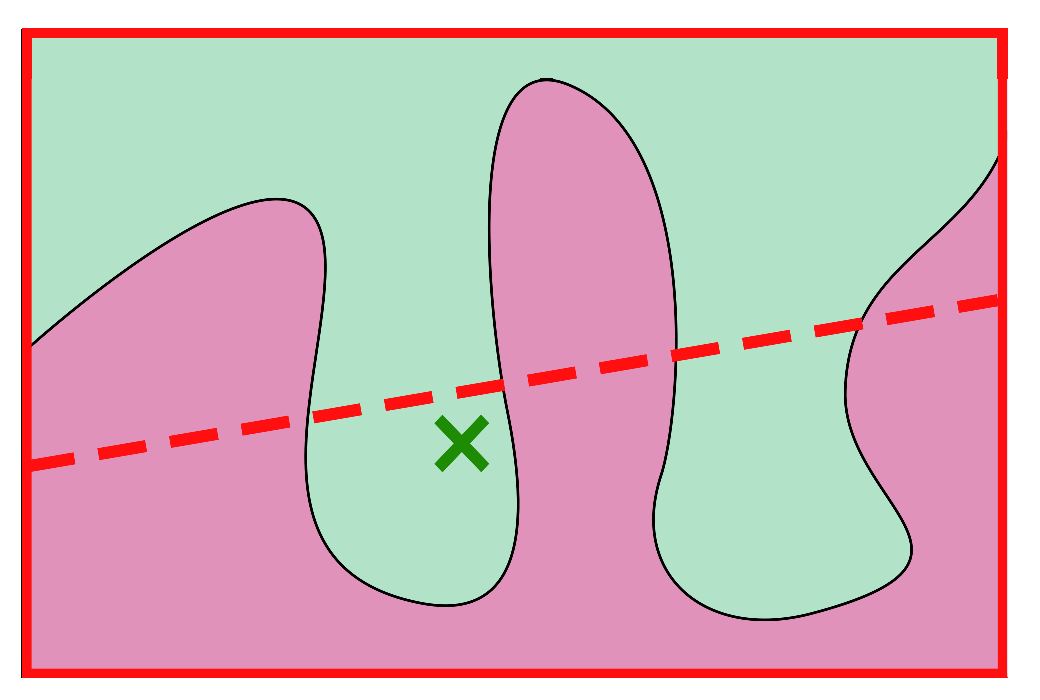
\includegraphics[width=0.31\textwidth]{img/visual-rlime1}
    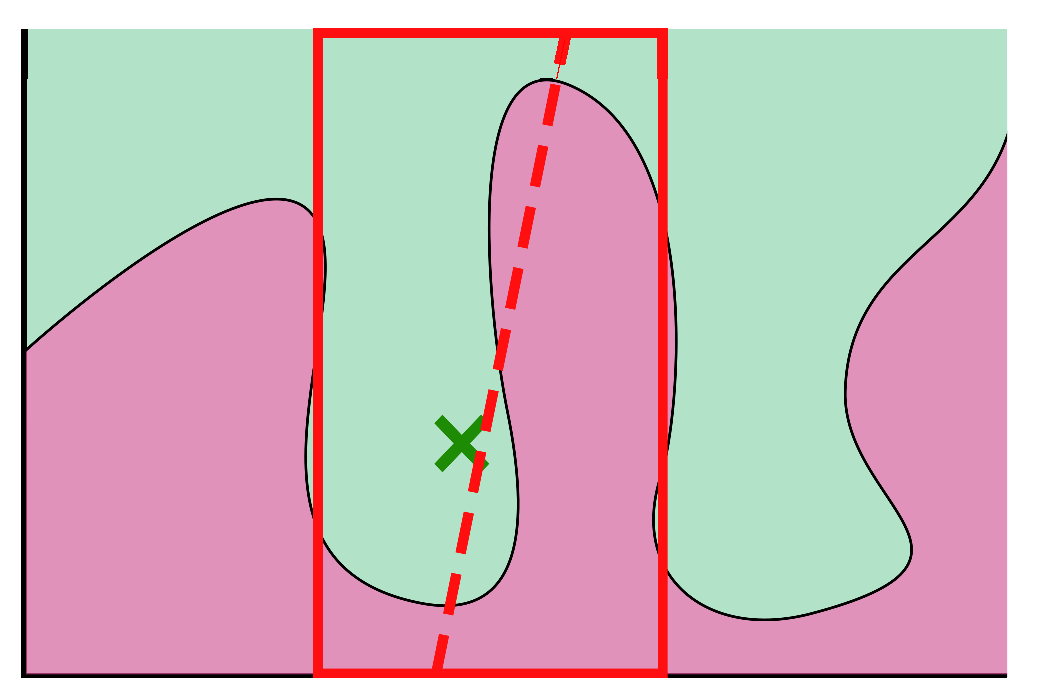
\includegraphics[width=0.31\textwidth]{img/visual-rlime2}
    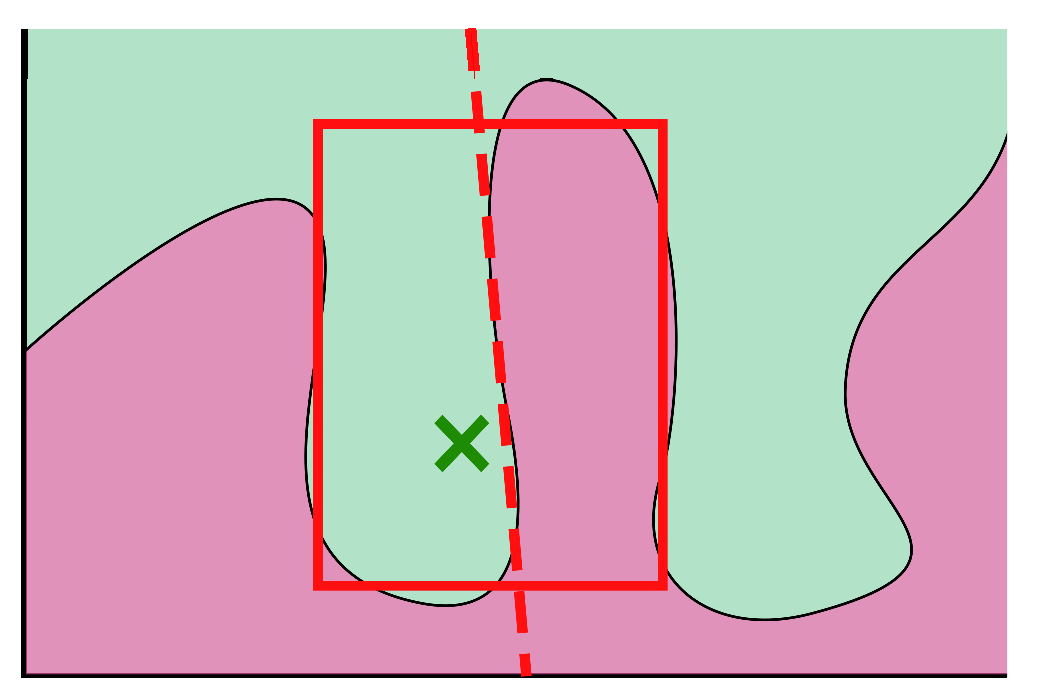
\includegraphics[width=0.31\textwidth]{img/visual-rlime3}
  \end{figure}
\end{frame}

\section{Experiments}

\subsection{Qualitative Evaluation}

\subsubsection{Setting}

\begin{frame}{}
  Visually compare LIME and R-LIME on the real dataset
  \begin{itemize}
    \item Use recidivism dataset\footfullcite{schmidt1988predicting}
    \item Train black-box classifier (random forest)
    \item Compare the output explanations of LIME and R-LIME
  \end{itemize}
\end{frame}

\def\index{0012}
\def\dir{src/rlime-paper/src/experiments/exp1}

\begin{frame}{}
  \renewcommand{\arraystretch}{0.80}
  \centering
  \footnotesize
  \begin{table}
    \begin{tabular}{p{14em}m{16em}}
      \toprule
      \csvreader[no head, late after line= \\]{%
        \dir/\index.csv
      }{}{\ifnum\thecsvrow=16\midrule\fi\csvcoli{} & \csvcolii}
      \bottomrule
    \end{tabular}
  \end{table}
\end{frame}


{%
\def\scale{0.42}

\subsubsection{Results --- LIME}
\begin{frame}{}
  LIME provides the importance of each feature to the prediction of the random forest
  \bigskip
  \begin{figure}[b]
    \hspace{-4em}
    \includegraphics[scale=\scale]{experiments/exp1/lime-\index}
  \end{figure}
\end{frame}

\subsubsection{Results --- R-LIME ($\tau=0.70$)}
\begin{frame}{}
  R-LIME provides not only the feature importance but also its application scope.

  It can be only applied to \underline{married} prisoners!
  \begin{figure}
    \hspace{-3.7em}
    \includegraphics[scale=\scale]{experiments/exp1/rlime-\index-70}
  \end{figure}
\end{frame}

\subsubsection{Results --- R-LIME ($\tau=0.90$)}
\begin{frame}{}
  Too low coverage $\rightarrow$ \underline{Limited generality}
  \begin{figure}
    \hspace{-4.5em}
    \includegraphics[scale=\scale]{experiments/exp1/rlime-\index-90}
  \end{figure}
\end{frame}
}

\subsection{Quantitative Evaluation}

\subsubsection{Setting}

\begin{frame}{}
  Compare local approximation accuracy of LIME and R-LIME
  \begin{itemize}
    \item Train random forest model on recidivism dataset
    \item Repeat the following steps against 100 instances
          \begin{itemize}
            \item Generate explanations of LIME and R-LIME
            \item Sample 10000 instances within the region of
                  the R-LIME explanation
            \item Calculate the local approximation accuracy of LIME and R-LIME
          \end{itemize}
  \end{itemize}
\end{frame}

\subsubsection{Results}
\begin{frame}{}
  \begin{figure}
    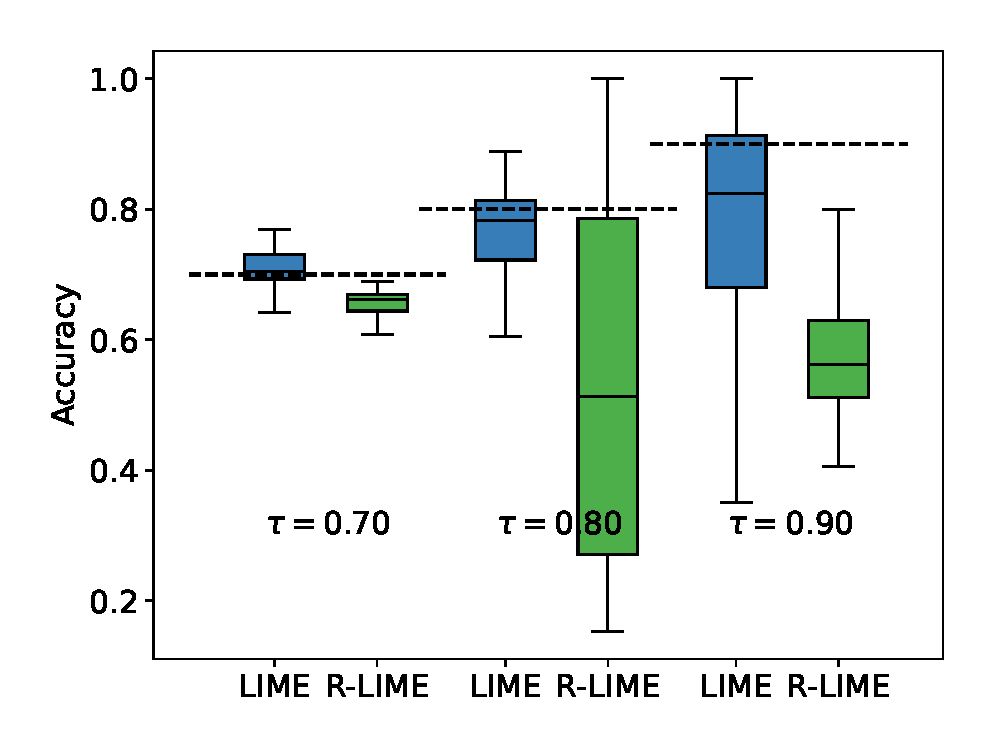
\includegraphics[height=142pt]{experiments/exp2/box_plot}
  \end{figure}
  \begin{itemize}
    \item R-LIME learns high-accuracy model adapted to the oprimized region
    \item LIME may not effectively approximize depending on how the region selected
  \end{itemize}
\end{frame}

\section{Discussion}

\begin{frame}{}
  Topics of Discussion
  \begin{itemize}
    \item Behavior for imbalanced label distribution
    \item Changes in reword distribution in best arm identification
    \item Parameter selection
  \end{itemize}
\end{frame}

\subsection{Behavior for Imbalanced Label Distribution}

\begin{frame}{}
  When the ratio of minority labels is less than $1-\tau$
  \begin{figure}
    \centering
    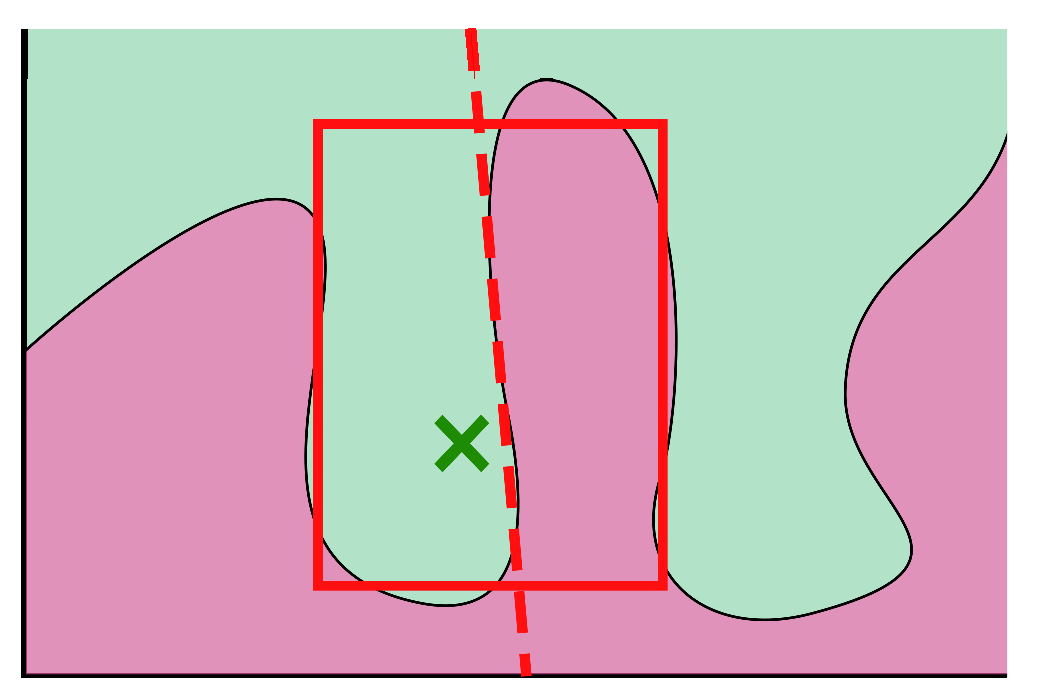
\includegraphics[width=0.39\textwidth]{img/visual-rlime3}
    \hspace{1em}
    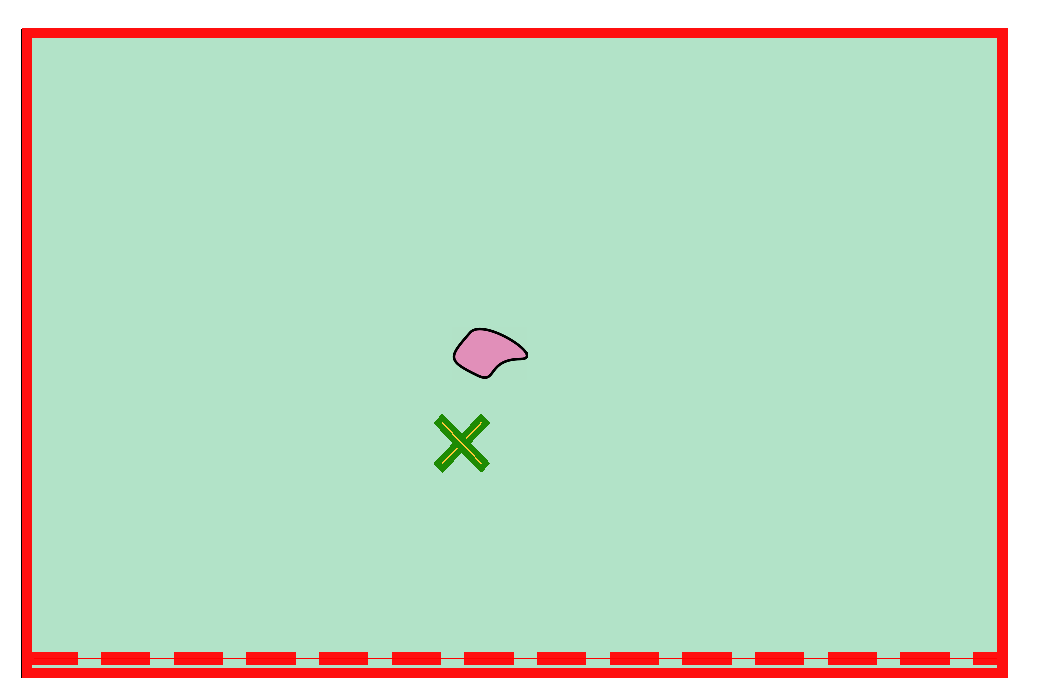
\includegraphics[width=0.4\textwidth]{img/visual-rlime-imbalanced}
  \end{figure}
  R-LIME covers the entire input space and always outputs the majority label
\end{frame}

\subsubsection{Possible solutions}

\begin{frame}{}
  \begin{itemize}
    \item Modify the loss function
          \begin{itemize}
            \item weighted logistic loss
            \item Focal Loss\footfullcite{lin2020focal}
          \end{itemize}
    \item Constraint on imbalanced label distribution
          \begin{itemize}
            \item add the following constraint
                  \begin{flalign*}
                    {\left(\mathbb{E}_{z\sim\mathcal{D}(z|A)}
                      [\mathbbm{1}_{f(z)=1}]-\frac{1}{2}\right)}^2<\mu
                  \end{flalign*}
          \end{itemize}
  \end{itemize}
\end{frame}

\subsection{Changes in Reword Distribution}

\begin{frame}{}
  Best arm identification using KL-LUCB algorithm\footfullcite{kaufmann2013information}
  \begin{columns}[]
    \begin{column}{0.65\textwidth}
      \begin{itemize}
        \item the original assumes constant reword distribution
        \item but in R-LIME, it changes with every update of the model after sampling
      \end{itemize}
    \end{column}
    \begin{column}{0.4\textwidth}
      \begin{figure}
        \centering
        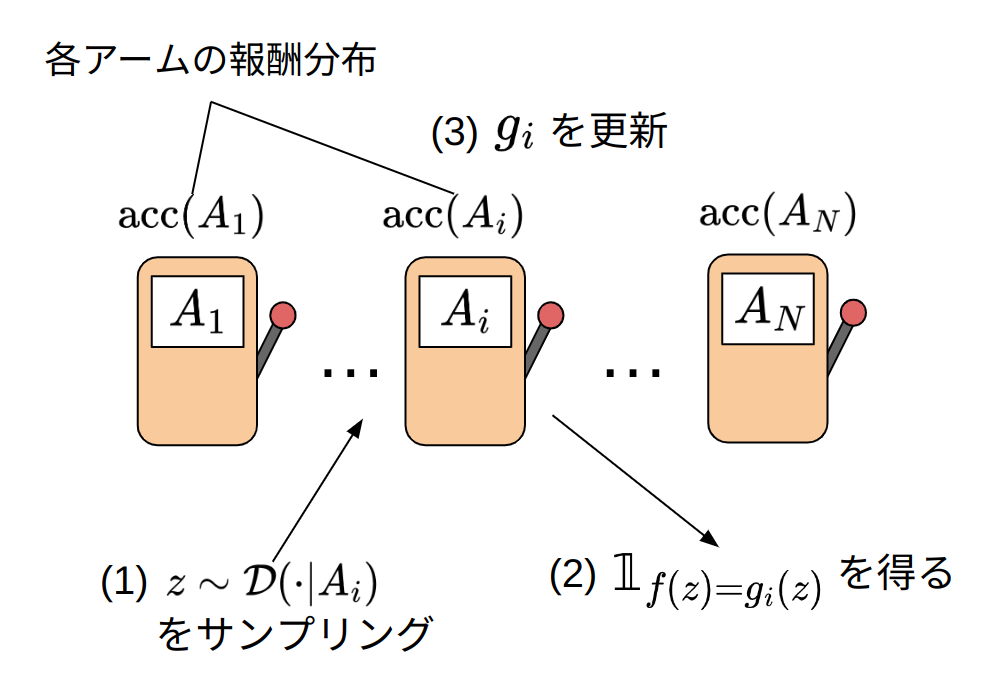
\includegraphics[width=0.9\textwidth]{bandit}
      \end{figure}
    \end{column}
  \end{columns}
\end{frame}

\subsubsection{Evaluation}

\begin{frame}{}
  \begin{table}
    \begin{tabular}{cccc}
  \toprule
                     & Estimated acc. & True acc. & Deviation \\
  \midrule
  Average            & .811           & .829      & .012      \\
  Standard Deviation & .018           & .023      & .017      \\
  \bottomrule
\end{tabular}

    \caption{Comparison of true accuracy and estimated accuracy by R-LIME}
  \end{table}

  Considering confidence level $1-\delta=0.95$,
  the deviation was relatively small.
\end{frame}

\section{Conclusion}

\begin{frame}{}
  \renewcommand{\arraystretch}{1.5}
  \tabcolsep=1.5em
  \begin{center}
    \begin{tabular}{cccc}
                          & LIME         & Anchor       & \textbf{R-LIME} \\
      \midrule
      Feature Importance  & \checkmark{} & $\times$     & \checkmark{}    \\
      Optimal Scope       & $\times$     & \checkmark{} & \checkmark{}    \\
      Interpretable Scope & $\times$     & \checkmark{} & \checkmark{}    \\
    \end{tabular}
  \end{center}
  \center{%
    \colorrect{green!20}{%
      Our methods achieves interpretability of both explanation and its scope!
    }
  }
\end{frame}

\renewcommand\appendixname{Appendix}
\appendix
\section{Appendix}

\begin{frame}
  \begin{algorithm}[H]
    \caption{R-LIME}
    \begin{algorithmic}[1]
      \Require{%
        Black-box model $f$, Target instance $x$,
        Distribution $\mathcal{D}$,
        Threshold $\tau$, Beam width $B$, Tolerance $\epsilon$,
        Confidence level $1-\delta$
      }
      \Ensure{%
        Rule $A^*$ satisfying Eq.~\eqref{eq:main-problem}
      }
      \State{$A^*\gets\textbf{null},\ \mathcal{A}_0\gets\emptyset,\ t\gets0$}
      % \Comment{%
      %   Initialize the set of candidate rules $\mathcal{A}_0$ to $\emptyset$
      % }
      \Comment{Initialize the set of candidate rules $\mathcal{A}_0$ to $\emptyset$}
      \While{$A^*=\textbf{null}$}
      \State$t\gets t+1$
      \State$\cands_t\gets$ \Call{GenerateCands}
      {$\mathcal{A}_{t-1}$}
      \State$\mathcal{A}_t\gets$ \Call{B-BestCands}
      {$\cands_{t},\mathcal{D},B,\epsilon,\delta$}
      \State$A^*\gets$ \Call{LargestCand}
      {$\mathcal{A}_t,\tau,\delta$}
      \EndWhile%
    \end{algorithmic}
  \end{algorithm}
  \vspace{-2em}
  \begin{equation}
    \tilde{A}=\underset{A\ s.t.
      \ P(\Prec(A)\ge\tau)\ge1-\delta,A(x)=1}
    {\arg\max}\operatorname{cov}(A)\label{eq:main-problem}
  \end{equation}
\end{frame}

\begin{frame}
  \begin{algorithm}[H]
    \caption{Generating new candidate rules}
    \begin{algorithmic}[1]
      \Function{GenerateCands}{$\mathcal{A},x$}
      \IIf{$\mathcal{A}=\emptyset$}{\Return{$\{\mathit{true}\}$}}
      \Comment{An initial empty rule always returns $\mathit{true}$}
      \State$\cands\gets\emptyset$
      \ForAll{$A\in\mathcal{A}$}
      \ForAll{$a\in (T(x)\setminus A)$}
      \State$\cands\gets\bar{\mathcal{A}}\cup(A\wedge a)$
      \Comment{Get a new rule by adding a new predicate $a$ to $A$}
      \EndFor%
      \EndFor%
      \State\Return{$\cands$}
      \EndFunction%
    \end{algorithmic}
  \end{algorithm}
\end{frame}

\begin{frame}
  \begin{algorithm}[H]
    \small
    \caption{%
      Searching rules with highest accuracy (KL-LUCB~\cite{kaufmann2013information})
    }
    \begin{algorithmic}[1]
      \Function{B-BestCands}{$\cands,\mathcal{D},B,\epsilon,\delta$}
      \State\textbf{initialize} $\Prec,\Prec_{u},\Prec_{l}$ for $\forall A\in\cands$
      \State$\mathcal{A}\gets\Call{B-ProvisionallyBestCands}{\cands}$
      \Comment{$B$ rules with highest accuracy}
      \State$A\gets\arg\min_{A\in\mathcal{A}}\Prec_{l}(A,\delta)$
      \Comment{The rule with the smallest lower bound}
      \State$A'\gets\arg\max_{A'\notin(\cands\setminus\mathcal{A})}\Prec_{u}(A',\delta)$
      \Comment{The rule with the largest upper bound}
      \While{$~\Prec_{u}(A',\delta)-\Prec_{l}(A,\delta)>\epsilon$}
      \State\textbf{sample} $z\sim\mathcal{D}(z|A),z'\sim\mathcal{D}(z'|A')$
      \State\textbf{update} $\Prec,\Prec_{u},\Prec_{l}$ for $A$ and $A'$
      \State$\mathcal{A}\gets\Call{B-ProvisionallyBestCands}{\cands}$
      \State$A\gets\arg\min_{A\in\mathcal{A}}\Prec_{l}(A,\delta)$
      \State$A'\gets\arg\max_{A'\notin(\cands\setminus\mathcal{A})}\Prec_{u}(A',\delta)$
      \EndWhile%
      % \State\algorithmicdo%
      % \State\myidt$\mathcal{A}\gets\Call{B-ProvisionallyBestCands}{\cands}$
      % \State\myidt$A\gets\arg\min_{A\in\mathcal{A}}\Prec_{l}(A)$
      % \State\myidt$A'\gets\arg\max_{A'\notin(\cands\setminus\mathcal{A})}\Prec_{u}(A')$
      % \State\myidt\textbf{sample} $z\sim\mathcal{D}(z|A),z'\sim\mathcal{D}(z'|A')$
      % \State\myidt\textbf{update} $\Prec,\Prec_{u},\Prec_{l}$ for $A$ and $A'$
      % \State\algorithmicwhile$~\Prec_{u}(A')-\Prec_{l}(A)>\epsilon$
      \State\Return{$\mathcal{A}$}
      \EndFunction%
    \end{algorithmic}
  \end{algorithm}
\end{frame}

\begin{frame}
  \begin{algorithm}[H]
    \caption{Searching a rule with highest coverage under constraint}
    \begin{algorithmic}[1]
      \Function{LargestCand}{$\mathcal{A},\tau,\delta$}
      \State$A^*\gets\textbf{null}$
      \Comment{If no rule satisfies the constraint, return $\textbf{null}$}
      \ForAll{$A\in\mathcal{A}$ s.t. $\Prec_{l}(A,\delta)>\tau$}
      \IIf{$\Cov(A)>\Cov(A^*)$}{$A^*\gets A$}
      \EndFor%
      \State\Return{$A^*$}
      \EndFunction%
    \end{algorithmic}
  \end{algorithm}
\end{frame}

\end{document}
